\section{Data flow}
\begin{frame}{Farm topology}{}
	\begin{itemize}
	  \item Only one single farm (L1 and L2 combined)
	  \item All transmissions via UDP/IP
	\end{itemize}
	\begin{center} 
		\includegraphics[width=10cm]{merged-star-engl}
	\end{center} 
\end{frame}

\begin{frame}{L1 eventbuilding}{}
	\begin{center} 
		\includegraphics[width=7cm]{dataflow-merged-gian-engl}
	\end{center} 
	\begin{block}{Every board must send one event to the same PC}
		Round robin table:
		\begin{itemize}
		  \item Send Events [0, N-1] to PC1
		  \item Send Event [N, 2N-1] to PC2
		  \item \ldots
		\end{itemize}
	\end{block}
\end{frame}

\begin{frame}{Load balancing}{}
	What if a PC crashes or the farm is inhomogeneous?
	\begin{block}{RR table should be updated burst wise}
		\begin{itemize}
		  \item Remove dead PCs out of the table
		  \item Put slow PCs less times into the table
		\end{itemize}
	\end{block}
\end{frame}

\begin{frame}{Data model for L0 data}{}
	\begin{center} 
		\includegraphics[width=9cm]{eb-data-model-engl}
	\end{center} 
\end{frame}

\begin{frame}{Eventbuilding}{}
	The number of event-parts (MEPEs) is constant for every source ID
	\\
	\begin{ergo}
		Parameter
		-~-L0DataSourceIDs=0x04:2,0x08:3,0x0C:1,\ldots
	\end{ergo}
	
	\\
	The framework will wait for two packets from 0x04, three packets from
	0x08\ldots before starting with processing L1.
	
\begin{figure}[htp]
\begin{center}
  \includegraphics[width=6cm]{MEP-engl}
  \caption{Multi Event Packet (MEP)}
\end{center}
\end{figure}
\end{frame}


\begin{frame}{CREAM request}{}
If the L1 triggerWord is not zero a trigger will be sent to the CREAMs within a
MTP. Following parameters control the L1 requests:
\begin{description}
  \item[maxTriggerPerL1MTP] Maximum number of triggers within one MTP.
  \item[maxL1TriggerDataRate] Maximum data rate the MTPs may be sent (in MBps).
\end{description}
\end{frame}

\begin{frame}[fragile]
	\frametitle{L2 eventbuilding and trigger}
	It is expected to get one packet from every CREAM. The CREAM IDs \textbf{and} crate IDs
	must be \textbf{consecutive}:
	\begin{description}
	  \item[CREAMCrates] Number of CREAMs for every crate. CREAMCrates=2,5,4 means
	  crate 0 has 2 CREAMs, crate 1 has 5\ldots
	\end{description}
	

\begin{figure}[htp]
\begin{center}
  \includegraphics[width=6cm]{CREAM-Data-engl}
  \caption{CREAM data packets}
\end{center}
\end{figure}


\end{frame}


\section{Implementation}
\begin{frame}{Circular buffers for parallelization}{}
	Bad performance with semaphores/mutexes \\
	$\Rightarrow$ Parallelization based on lockless queues:
	\begin{center} 
		\includegraphics[width=10cm]{consumer-producer-queue}
	\end{center} 
\end{frame}

\begin{frame}{Software overview}{}
	\begin{center} 
		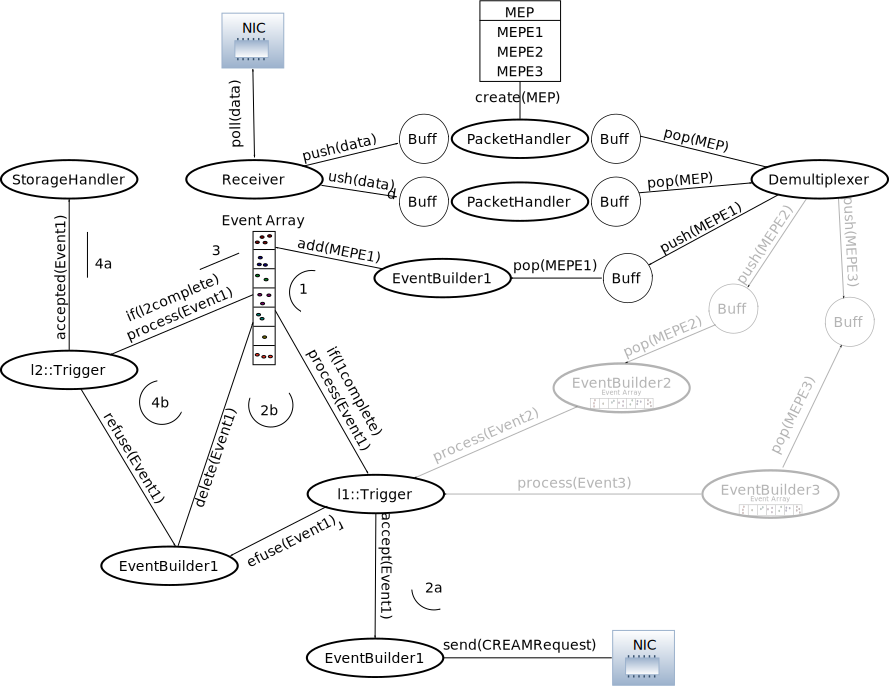
\includegraphics[width=9cm]{farm-concept}
	\end{center} 
\end{frame}

\begin{frame}{Polling and packet handling}{}
	Memcpy to userland, create data structures, check integrity
	\begin{center} 
		\includegraphics[width=9cm]{farm-concept1}
	\end{center} 
\end{frame}

\begin{frame}{EB distribution}{}
	N event builder: Move MEPE M to event builder M mod N
	\begin{center} 
		\includegraphics[width=9cm]{farm-concept2}
	\end{center} 
\end{frame}

\begin{frame}{Eventbuilding}{}
	Add MEPE to an existing (empty) Event-object 
	\begin{center} 
		\includegraphics[width=9cm]{farm-concept3}
	\end{center} 
\end{frame}

\begin{frame}{L1 Trigger}{}
	Call TriggerProcessor if all MEPEs have been received. Delete event if trigger
	word is zero\ldots
	\begin{center} 
		\includegraphics[width=9cm]{farm-concept4}
	\end{center} 
\end{frame}

\begin{frame}[fragile]
\frametitle{Trigger software interface}
\begin{lstlisting}[frame=trBL,caption={}]{hallowelt}
const uint16_t TriggerProcessor::computeL1(Event* event) {
    uint16_t triggerWord=0;
    Subevent* MUVEvents = event->getL0SubeventBySourceID(0x28);
    for (uint16_t i = 0; i < subevent->getNumberOfParts(); i++) {
        MEPEvent* e = subevent->getEventPart(i);
        u_char* rawData = e->getDataWithHeader();
        //... do something
    } 
    return triggerWord;	
}
\end{lstlisting}
\end{frame}

\begin{frame}{L1 MTP distribution}{}
	\ldots or push event to L1DistributionHandler that will send MTP
	\begin{center} 
		\includegraphics[width=9cm]{farm-concept5}
	\end{center} 
\end{frame}

\begin{frame}{L2 event building}{}
	Do the same with LKr data
	\begin{center} 
		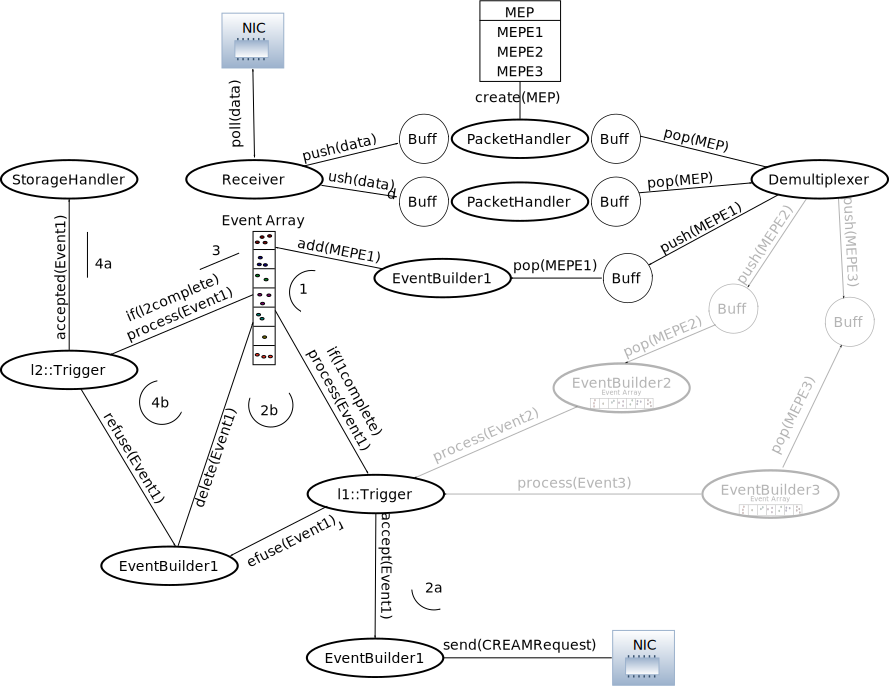
\includegraphics[width=9cm]{farm-concept}
	\end{center} 
\end{frame}


\begin{frame}[fragile]
\frametitle{L2 trigger}
\begin{lstlisting}[frame=trBL,caption={}]{hallowelt}
const uint8_t TriggerProcessor::computeL2(Event* event) {
	LKREvent lkrEvent = event->getLKrEvent(crateID, CREAMID);
    u_char* rawData = e->getDataWithHeader();
	...
	return L2TriggerWord;
}
\end{lstlisting}

\end{frame}


		
\begin{frame}{Load (upper limits)}{}
Full Speed L1/L2 simulation:

\begin{table}
	\begin{tabular}{c c c}
		Process	& Threads	& CPU Load \\
		\hline
		Receiver+EB		&	1	&	$<80$\% \\
		PacketHandler	&	2	&	$<140$\% \\
		EventBuilder	&	11	&	$<300$\%	\\
	\end{tabular}
	\end{table}
	\begin{ergo}
		Less than 18\% of the CPU for housekeeping $\Rightarrow$ more than 82\%
		remaining for L1 and L2 Trigger processing
	\end{ergo}
\end{frame}


\section{L1 MTP distribution}
\begin{frame}{L1 MTP distribution via multicast}{}
	How to let one PC send MTPs to every CREAM:
	\begin{itemize}
	  \item Multicast groups are defined by addresses (224.0.0.0 to
	  239.255.255.25)
	  \item The receiver can join a group via IGMP
	  \item The sender needs to send to the group-IP via a special MAC address
	  \item The switch must be configured to listen to IGMP
	\end{itemize}
\end{frame}

\section{Monitoring}
\begin{frame}{Monitoring}{}
	\begin{itemize}
	  \item Every monitored vaiable (e.g. CPU load, data rates, trigger word
	distribution\ldots) is sent to a central mySQL DB
	\item The frequency is adjustable by -~-monitorUpdateTime
	\item The database can be used for heartbeats
	\item New monitored variables are added within one line of code
	\end{itemize}
	
		\begin{ergo}
		I already implemented a small GWT based web frontend to visualize the
		data to  
	\end{ergo}
	
	\begin{center}
	  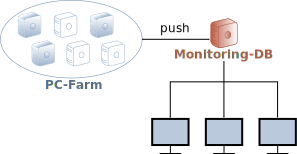
\includegraphics[width=5cm]{monitoring}
	\end{center}
\end{frame}


\section{Outlook}
\begin{frame}{Outlook}{}
	\begin{itemize}
	  \item 3 weeks remaining
	  \item IP segmentation still to be implemented
	  \item Detailed specification under construction (apart from my german
	  thesis)
	  \vspace{1cm}
	  \item Any idea about a nice Ph.D. topic?
	\end{itemize}
\end{frame}